\documentclass[a4paper]{article}

%================================================================================================================================
%
% Packages
%
%================================================================================================================================

\usepackage[T1]{fontenc} 	% pour caractères accentués
\usepackage[utf8]{inputenc}  % encodage utf8
\usepackage[french]{babel}	% langue : français
\usepackage{fourier}			% caractères plus lisibles
\usepackage[dvipsnames]{xcolor} % couleurs
\usepackage{fancyhdr}		% réglage header footer
\usepackage{needspace}		% empêcher sauts de page mal placés
\usepackage{graphicx}		% pour inclure des graphiques
\usepackage{enumitem,cprotect}		% personnalise les listes d'items (nécessaire pour ol, al ...)
\usepackage{hyperref}		% Liens hypertexte
\usepackage{pstricks,pst-all,pst-node,pstricks-add,pst-math,pst-plot,pst-tree,pst-eucl} % pstricks
\usepackage[a4paper,includeheadfoot,top=2cm,left=3cm, bottom=2cm,right=3cm]{geometry} % marges etc.
\usepackage{comment}			% commentaires multilignes
\usepackage{amsmath,environ} % maths (matrices, etc.)
\usepackage{amssymb,makeidx}
\usepackage{bm}				% bold maths
\usepackage{tabularx}		% tableaux
\usepackage{colortbl}		% tableaux en couleur
\usepackage{fontawesome}		% Fontawesome
\usepackage{environ}			% environment with command
\usepackage{fp}				% calculs pour ps-tricks
\usepackage{multido}			% pour ps tricks
\usepackage[np]{numprint}	% formattage nombre
\usepackage{tikz,tkz-tab} 			% package principal TikZ
\usepackage{pgfplots}   % axes
\usepackage{mathrsfs}    % cursives
\usepackage{calc}			% calcul taille boites
\usepackage[scaled=0.875]{helvet} % font sans serif
\usepackage{svg} % svg
\usepackage{scrextend} % local margin
\usepackage{scratch} %scratch
\usepackage{multicol} % colonnes
%\usepackage{infix-RPN,pst-func} % formule en notation polanaise inversée
\usepackage{listings}

%================================================================================================================================
%
% Réglages de base
%
%================================================================================================================================

\lstset{
language=Python,   % R code
literate=
{á}{{\'a}}1
{à}{{\`a}}1
{ã}{{\~a}}1
{é}{{\'e}}1
{è}{{\`e}}1
{ê}{{\^e}}1
{í}{{\'i}}1
{ó}{{\'o}}1
{õ}{{\~o}}1
{ú}{{\'u}}1
{ü}{{\"u}}1
{ç}{{\c{c}}}1
{~}{{ }}1
}


\definecolor{codegreen}{rgb}{0,0.6,0}
\definecolor{codegray}{rgb}{0.5,0.5,0.5}
\definecolor{codepurple}{rgb}{0.58,0,0.82}
\definecolor{backcolour}{rgb}{0.95,0.95,0.92}

\lstdefinestyle{mystyle}{
    backgroundcolor=\color{backcolour},   
    commentstyle=\color{codegreen},
    keywordstyle=\color{magenta},
    numberstyle=\tiny\color{codegray},
    stringstyle=\color{codepurple},
    basicstyle=\ttfamily\footnotesize,
    breakatwhitespace=false,         
    breaklines=true,                 
    captionpos=b,                    
    keepspaces=true,                 
    numbers=left,                    
xleftmargin=2em,
framexleftmargin=2em,            
    showspaces=false,                
    showstringspaces=false,
    showtabs=false,                  
    tabsize=2,
    upquote=true
}

\lstset{style=mystyle}


\lstset{style=mystyle}
\newcommand{\imgdir}{C:/laragon/www/newmc/assets/imgsvg/}
\newcommand{\imgsvgdir}{C:/laragon/www/newmc/assets/imgsvg/}

\definecolor{mcgris}{RGB}{220, 220, 220}% ancien~; pour compatibilité
\definecolor{mcbleu}{RGB}{52, 152, 219}
\definecolor{mcvert}{RGB}{125, 194, 70}
\definecolor{mcmauve}{RGB}{154, 0, 215}
\definecolor{mcorange}{RGB}{255, 96, 0}
\definecolor{mcturquoise}{RGB}{0, 153, 153}
\definecolor{mcrouge}{RGB}{255, 0, 0}
\definecolor{mclightvert}{RGB}{205, 234, 190}

\definecolor{gris}{RGB}{220, 220, 220}
\definecolor{bleu}{RGB}{52, 152, 219}
\definecolor{vert}{RGB}{125, 194, 70}
\definecolor{mauve}{RGB}{154, 0, 215}
\definecolor{orange}{RGB}{255, 96, 0}
\definecolor{turquoise}{RGB}{0, 153, 153}
\definecolor{rouge}{RGB}{255, 0, 0}
\definecolor{lightvert}{RGB}{205, 234, 190}
\setitemize[0]{label=\color{lightvert}  $\bullet$}

\pagestyle{fancy}
\renewcommand{\headrulewidth}{0.2pt}
\fancyhead[L]{maths-cours.fr}
\fancyhead[R]{\thepage}
\renewcommand{\footrulewidth}{0.2pt}
\fancyfoot[C]{}

\newcolumntype{C}{>{\centering\arraybackslash}X}
\newcolumntype{s}{>{\hsize=.35\hsize\arraybackslash}X}

\setlength{\parindent}{0pt}		 
\setlength{\parskip}{3mm}
\setlength{\headheight}{1cm}

\def\ebook{ebook}
\def\book{book}
\def\web{web}
\def\type{web}

\newcommand{\vect}[1]{\overrightarrow{\,\mathstrut#1\,}}

\def\Oij{$\left(\text{O}~;~\vect{\imath},~\vect{\jmath}\right)$}
\def\Oijk{$\left(\text{O}~;~\vect{\imath},~\vect{\jmath},~\vect{k}\right)$}
\def\Ouv{$\left(\text{O}~;~\vect{u},~\vect{v}\right)$}

\hypersetup{breaklinks=true, colorlinks = true, linkcolor = OliveGreen, urlcolor = OliveGreen, citecolor = OliveGreen, pdfauthor={Didier BONNEL - https://www.maths-cours.fr} } % supprime les bordures autour des liens

\renewcommand{\arg}[0]{\text{arg}}

\everymath{\displaystyle}

%================================================================================================================================
%
% Macros - Commandes
%
%================================================================================================================================

\newcommand\meta[2]{    			% Utilisé pour créer le post HTML.
	\def\titre{titre}
	\def\url{url}
	\def\arg{#1}
	\ifx\titre\arg
		\newcommand\maintitle{#2}
		\fancyhead[L]{#2}
		{\Large\sffamily \MakeUppercase{#2}}
		\vspace{1mm}\textcolor{mcvert}{\hrule}
	\fi 
	\ifx\url\arg
		\fancyfoot[L]{\href{https://www.maths-cours.fr#2}{\black \footnotesize{https://www.maths-cours.fr#2}}}
	\fi 
}


\newcommand\TitreC[1]{    		% Titre centré
     \needspace{3\baselineskip}
     \begin{center}\textbf{#1}\end{center}
}

\newcommand\newpar{    		% paragraphe
     \par
}

\newcommand\nosp {    		% commande vide (pas d'espace)
}
\newcommand{\id}[1]{} %ignore

\newcommand\boite[2]{				% Boite simple sans titre
	\vspace{5mm}
	\setlength{\fboxrule}{0.2mm}
	\setlength{\fboxsep}{5mm}	
	\fcolorbox{#1}{#1!3}{\makebox[\linewidth-2\fboxrule-2\fboxsep]{
  		\begin{minipage}[t]{\linewidth-2\fboxrule-4\fboxsep}\setlength{\parskip}{3mm}
  			 #2
  		\end{minipage}
	}}
	\vspace{5mm}
}

\newcommand\CBox[4]{				% Boites
	\vspace{5mm}
	\setlength{\fboxrule}{0.2mm}
	\setlength{\fboxsep}{5mm}
	
	\fcolorbox{#1}{#1!3}{\makebox[\linewidth-2\fboxrule-2\fboxsep]{
		\begin{minipage}[t]{1cm}\setlength{\parskip}{3mm}
	  		\textcolor{#1}{\LARGE{#2}}    
 	 	\end{minipage}  
  		\begin{minipage}[t]{\linewidth-2\fboxrule-4\fboxsep}\setlength{\parskip}{3mm}
			\raisebox{1.2mm}{\normalsize\sffamily{\textcolor{#1}{#3}}}						
  			 #4
  		\end{minipage}
	}}
	\vspace{5mm}
}

\newcommand\cadre[3]{				% Boites convertible html
	\par
	\vspace{2mm}
	\setlength{\fboxrule}{0.1mm}
	\setlength{\fboxsep}{5mm}
	\fcolorbox{#1}{white}{\makebox[\linewidth-2\fboxrule-2\fboxsep]{
  		\begin{minipage}[t]{\linewidth-2\fboxrule-4\fboxsep}\setlength{\parskip}{3mm}
			\raisebox{-2.5mm}{\sffamily \small{\textcolor{#1}{\MakeUppercase{#2}}}}		
			\par		
  			 #3
 	 		\end{minipage}
	}}
		\vspace{2mm}
	\par
}

\newcommand\bloc[3]{				% Boites convertible html sans bordure
     \needspace{2\baselineskip}
     {\sffamily \small{\textcolor{#1}{\MakeUppercase{#2}}}}    
		\par		
  			 #3
		\par
}

\newcommand\CHelp[1]{
     \CBox{Plum}{\faInfoCircle}{À RETENIR}{#1}
}

\newcommand\CUp[1]{
     \CBox{NavyBlue}{\faThumbsOUp}{EN PRATIQUE}{#1}
}

\newcommand\CInfo[1]{
     \CBox{Sepia}{\faArrowCircleRight}{REMARQUE}{#1}
}

\newcommand\CRedac[1]{
     \CBox{PineGreen}{\faEdit}{BIEN R\'EDIGER}{#1}
}

\newcommand\CError[1]{
     \CBox{Red}{\faExclamationTriangle}{ATTENTION}{#1}
}

\newcommand\TitreExo[2]{
\needspace{4\baselineskip}
 {\sffamily\large EXERCICE #1\ (\emph{#2 points})}
\vspace{5mm}
}

\newcommand\img[2]{
          \includegraphics[width=#2\paperwidth]{\imgdir#1}
}

\newcommand\imgsvg[2]{
       \begin{center}   \includegraphics[width=#2\paperwidth]{\imgsvgdir#1} \end{center}
}


\newcommand\Lien[2]{
     \href{#1}{#2 \tiny \faExternalLink}
}
\newcommand\mcLien[2]{
     \href{https~://www.maths-cours.fr/#1}{#2 \tiny \faExternalLink}
}

\newcommand{\euro}{\eurologo{}}

%================================================================================================================================
%
% Macros - Environement
%
%================================================================================================================================

\newenvironment{tex}{ %
}
{%
}

\newenvironment{indente}{ %
	\setlength\parindent{10mm}
}

{
	\setlength\parindent{0mm}
}

\newenvironment{corrige}{%
     \needspace{3\baselineskip}
     \medskip
     \textbf{\textsc{Corrigé}}
     \medskip
}
{
}

\newenvironment{extern}{%
     \begin{center}
     }
     {
     \end{center}
}

\NewEnviron{code}{%
	\par
     \boite{gray}{\texttt{%
     \BODY
     }}
     \par
}

\newenvironment{vbloc}{% boite sans cadre empeche saut de page
     \begin{minipage}[t]{\linewidth}
     }
     {
     \end{minipage}
}
\NewEnviron{h2}{%
    \needspace{3\baselineskip}
    \vspace{0.6cm}
	\noindent \MakeUppercase{\sffamily \large \BODY}
	\vspace{1mm}\textcolor{mcgris}{\hrule}\vspace{0.4cm}
	\par
}{}

\NewEnviron{h3}{%
    \needspace{3\baselineskip}
	\vspace{5mm}
	\textsc{\BODY}
	\par
}

\NewEnviron{margeneg}{ %
\begin{addmargin}[-1cm]{0cm}
\BODY
\end{addmargin}
}

\NewEnviron{html}{%
}

\begin{document}
\meta{url}{/exercices/cout-marginal-bac-blanc-es-l-sujet-3-maths-cours-2018/}
\meta{pid}{10473}
\meta{titre}{Coût marginal - Bac blanc ES/L Sujet 3 - Maths-cours 2018}
\meta{type}{exercices}
%
\begin{h2}Exercice 1 (5 points)\end{h2}
\par
Une entreprise fabrique une boisson conditionnée en bouteille d'un litre.
\par
Le coût total, exprimé en euros est donné par la fonction $C_t$ :
\[ C_t(x)=4x^3-20x^2+80x+100. \]
où $x$ représente le volume exprimé en centaines de litres, $x$ variant dans l'intervalle $[0~;~5]$.
\par
Le graphique ci-après affiche la représentation graphique $\mathscr{C}$ de la fonction $C_t$ dans un repère orthogonal.
\par
Le point $A$ est le point de la courbe $\mathscr{C}$ d'abscisse 5 et $B$ un point d'inflexion de cette courbe.
\par
$T_1$ et $T_2$ sont les tangentes à $\mathscr{C}$ respectivement aux points $A$ et $B$.
\par
\begin{center}
     \begin{extern}%width="550" alt="Graphique coût marginal"
          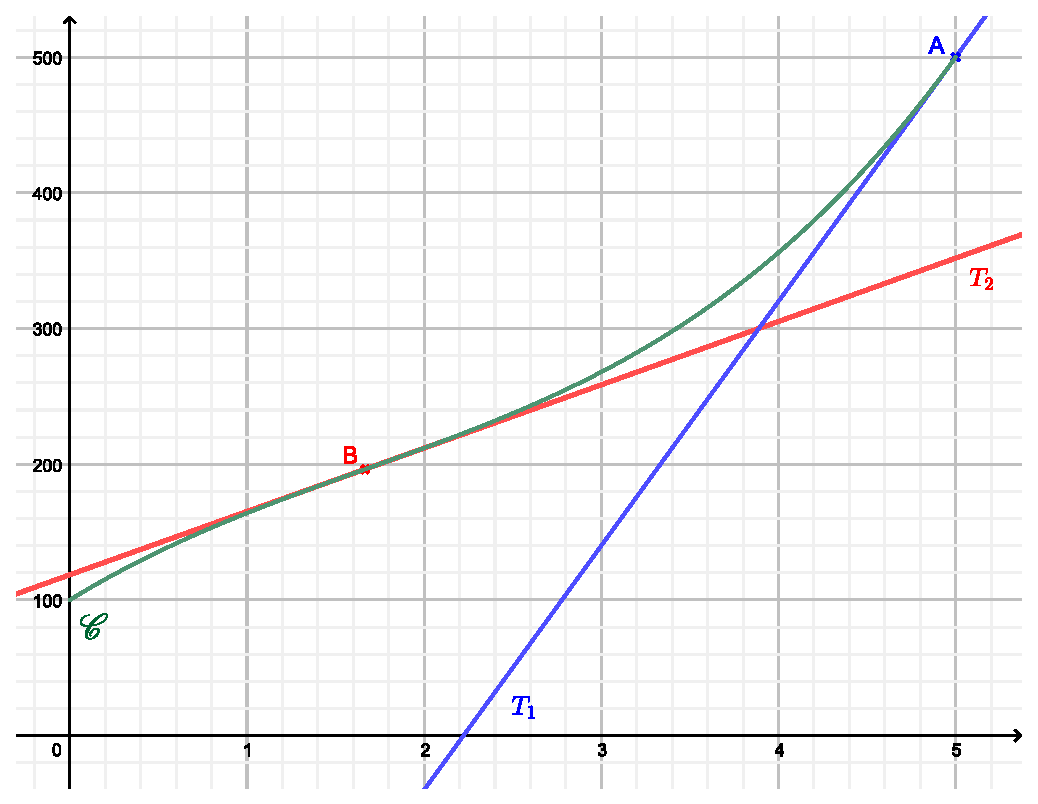
\includegraphics[width=0.9\textwidth]{images/BBESL-s3-1-1}% gbb 1 unite=3cm
     \end{extern}
\end{center}
\par
%============================================================================================================================
%
\TitreC{Partie A}
%
%============================================================================================================================
\par
\begin{enumerate}
     \item
     Les coûts fixes sont les coûts que supporte l'entreprise même lorsque la production est nulle.
     \par
     \`A l'aide du graphique ou de la formule définissant $C_t$, déterminer les coûts fixes puis le coût pour une production de 500 litres.
     \item
     Le coût marginal est égal au coût de fabrication d'une unité supplémentaire.
     \par
     On rappelle que l'on peut assimiler le coût marginal à la dérivée du coût total.
     \par
     Par lecture graphique, donner une estimation du coefficient directeur à la courbe $\mathscr{C}$ au point $A$ d'abscisse 5.
     \par
     En déduire une estimation du coût marginal pour une production de 500 litres.
     \item
     Donner, par lecture graphique, une estimation de l'intervalle sur lequel la fonction $C_t$ est convexe et une estimation de l'intervalle sur lequel la fonction $C_t$ est concave.
     \item
     \`A l'aide du graphique, estimer la valeur minimum du coût marginal.
     \par
\end{enumerate}
\par
%============================================================================================================================
%
\TitreC{Partie B}
%
%============================================================================================================================
\par
\begin{enumerate}
     \item
     Pour $x$ appartenant à l'intervalle $[0~;~5]$, exprimer le coût marginal $C_m(x)$ en fonction de $x$.
     \item
     Déterminer les coordonnées exactes du point $B$.
     \par
     Retrouver, par le calcul, la valeur minimum du coût marginal.
     \par
\end{enumerate}
\begin{corrige}
     %============================================================================================================================
     %
     \TitreC{Partie A}
     %
     %============================================================================================================================
     \par
     \begin{enumerate}
          \item %1
          Les coûts fixes sont égaux à $C_t(0)$ :
          \par
          $C_t(0)=4 \times 0^3 -20 \times 0^2 + 80 \times 0 + 100 = 100$
          \par
          Les coûts fixes sont de \textbf{100 euros}.
          \par
          Pour une production de 500 litres, soit 5 centaines de litres, le coût total est égal à :
          \par
          $C_t(5)=4 \times 5^3 -20 \times 5^2 + 80 \times 5 + 100 = 500$
          \par
          Le coût total pour une production de 500 litres est égal à \textbf{500 euros}.
          \item %2
          La tangente en $A$ à la courbe $\mathscr{C}$ est la droite $T_1$. Cette droite passe par le point $A(5~;~500)$ et passe par un point $M$ de coordonnées proches de $(4~;~320)$.
          \par
          Le coefficient directeur $a$ de cette tangente est donc approximativement :
          \par
          $a=\dfrac{y_M-y_A}{x_M-x_A}=\dfrac{500-320}{5-4}=180$
          \par
          Le coût marginal $C_m(5)$ pour une production de 500 litres est égal au nombre dérivé $C'_t(5)$. Or, ce nombre est le coefficient directeur de la tangente au point $A$.
          \par
          \cadre{rouge}{À retenir}{
               Le \textbf{coefficient directeur de la tangente} à la courbe représentative de $f$ au point d'\textbf{abscisse} $\alpha$ est égal à $f'(\alpha)$.
          }
          \par
          Le coût marginal pour une production de 500 litres est donc approximativement égal à \textbf{180 euros}.
          \item %3
          Notons $x_B$ l'abscisse du point $B$.
          \par
          Par lecture graphique, on voit que la fonction $C_t$ est concave sur l'intervalle $[0~;~x_B]$ et convexe sur l'intervalle $[x_B~;~5]$.
          \par
          On constate également que les coordonnées du point d'inflexion $B$ sont approximativement $(1,7~;~195)$.
          \par
          On peut donc estimer que la fonction $C_t$ est \textbf{concave sur l'intervalle} $\bm{[0~;~1,7]}$ et \textbf{convexe sur l'intervalle} $\bm{[1,7~;~5]}$.
          \par
          \cadre{rouge}{À retenir}{
               Une fonction est \textbf{convexe} si et seulement si sa courbe représentative est située \textbf{au-dessus de ses tangentes} (courbe en \og $\cup$ \fg{}).
               \par
               Une fonction est \textbf{concave} si et seulement si sa courbe représentative est située \textbf{au-dessous de ses tangentes} (courbe en \og $\cap$ \fg{}).
               \par
               Un \textbf{point d'inflexion} est un point où la fonction \textbf{change de convexité}. En ce point, la tangente \og traverse \fg{} la courbe.
          }
          \item
          La fonction $C_t$ est convexe si et seulement si sa fonction dérivée $C'_t$ (identique à la fonction $C_m$) est croissante.
          \par
          \cadre{rouge}{À retenir}{
               Si $f$ est une fonction deux fois dérivable sur un intervalle $I$, les propositions suivantes sont équivalentes :
               \par
               \begin{itemize}
                    \item
                    la fonction $f$ est \textbf{connexe} sur $I$;
                    \item
                    la fonction dérivée $f'$ est \textbf{croissante} sur $I$;
                    \item
                    la fonction dérivée seconde $f''$ est \textbf{positive} sur $I$;
               \end{itemize}
\medskip
               De même, les propositions suivantes sont équivalentes :
               \par
               \begin{itemize}
                    \item
                    la fonction $f$ est \textbf{concave} sur $I$;
                    \item
                    la fonction dérivée $f'$ est \textbf{décroissante} sur $I$;
                    \item
                    la fonction dérivée seconde $f''$ est \textbf{négative} sur $I$;
               \end{itemize}
          }
          \par
          D'après la question précédente on peut tracer le tableau ci-après :
          \par
          %:-+-+-+-+- Engendré par : http://math.et.info.free.fr/TikZ/TableauxVariations/
          \begin{center}
               \begin{extern}%width="400" alt="tableau de variations coût marginal"
                    \begin{tikzpicture}[scale=0.875]
                         % Styles
                         \tikzstyle{cadre}=[thin]
                         \tikzstyle{fleche}=[->,>=latex,thin]
                         \tikzstyle{nondefini}=[lightgray]
                         % Dimensions Modifiables
                         \def\Lrg{1.5}
                         \def\HtX{1}
                         \def\HtY{0.5}
                         % Dimensions Calculées
                         \def\lignex{-0.5*\HtX}
                         \def\lignef{-1.5*\HtX}
                         \def\separateur{-0.5*\Lrg}
                         % Largeur du tableau
                         \def\gauche{-2*\Lrg}
                         \def\droite{4.5*\Lrg}
                         % Hauteur du tableau
                         \def\haut{0.5*\HtX}
                         \def\bas{-2.5*\HtX-2*\HtY}
                         % Ligne de l'abscisse : x
                         \node at (-1.3*\Lrg,0) {$x$};
                         \node at (0*\Lrg,0) {$0$};
                         \node at (2*\Lrg,0) {$x_B$};
                         \node at (4*\Lrg,0) {$5$};
                         % Ligne de la dérivée : f'(x)
                         \node at (-1.3*\Lrg,-1*\HtX) {$C_t$};
                         \node at (0*\Lrg,-1*\HtX) {$\ $};
                         \node at (1*\Lrg,-1*\HtX) {$\text{concave}$};
                         \node at (2*\Lrg,-1*\HtX) {$\ $};
                         \node at (3*\Lrg,-1*\HtX) {$\text{convexe}$};
                         \node at (4*\Lrg,-1*\HtX) {$\ $};
                         % Ligne de la fonction : f(x)
                         \node  at (-1.3*\Lrg,{-2*\HtX+(-1)*\HtY}) {$C'_t=C_m$};
                         \node (f1) at (0*\Lrg,{-2*\HtX+(0)*\HtY}) {$\ $};
                         \node (f2) at (2*\Lrg,{-2*\HtX+(-2)*\HtY}) {$\ $};
                         \node (f3) at (4*\Lrg,{-2*\HtX+(0)*\HtY}) {$\ $};
                         % Flèches
                         \draw[fleche] (f1) -- (f2);
                         \draw[fleche] (f2) -- (f3);
                         % Encadrement
                         \draw[cadre] (\separateur,\haut) -- (\separateur,\bas);
                         \draw[cadre] (\gauche,\haut) rectangle  (\droite,\bas);
                         \draw[cadre] (\gauche,\lignex) -- (\droite,\lignex);
                         \draw[cadre] (\gauche,\lignef) -- (\droite,\lignef);
                    \end{tikzpicture}
               \end{extern}
          \end{center}
          Le coût marginal est minimal pour $x=x_B \approx 1,7$.
          \par
          Ce minimum vaut $C_m(x_B)=C'_t(x_B)$.
          \par
          Pour déterminer la valeur de $C'_t(x_B)$, on procède comme à la question \textbf{2.}
          \par
          $C'_t(x_B)$ est le coefficient directeur de la tangente $T_2$ à la courbe $\mathscr{C}$ au point $B$.
          \par
          Cette tangente passe approximativement par les points de coordonnées $(0~;~120)$ et $(1,7~;~195)$.
          \par
          On a donc :
          \par
          $C'_t(x_B) \approx \dfrac{195-120}{1,7-0} \approx 44$
          \par
          Le coût marginal minimal peut être estimé à \textbf{44 euros}.
          \par
          \textit{Remarque : il ne s'agit que d'une estimation. Vous pouvez tout à fait trouver un résultat légèrement différent. La valeur exacte, calculée dans la partie B, est comprise entre 46 et 47 euros.}
          \par
     \end{enumerate}
     \par
     %============================================================================================================================
     %
     \TitreC{Partie B}
     %
     %============================================================================================================================
     \par
     \begin{enumerate}
          \item
          Pour $x$ appartenant à l'intervalle $[0~;~5]$ :
          \par
          $C_m(x)=C'_t(x)=4 \times 3x^2-20 \times 2x + 80 = 12 x^2-40x+ 80$
          \item
          Le point $B$ est le point d'inflexion de la courbe $\mathscr{C}$.
          Son abscisse correspond à la valeur de $x$ pour laquelle $C''_t(x)$ s'annule et change de signe.
          Or :
          \par
          $C''_t(x)=C'_m(x)=12 \times 2x-40=24x-40$
          \par
          $C''_t$ est une fonction affine qui s'annule et change de signe pour ${x=\dfrac{40}{24}=\dfrac{5}{3}}$.
          \par
          Le point $B$ a donc pour abscisse $\dfrac{5}{3}$.
          \par
          L'ordonnée de $B$ est :
          \par
          $C_t\left(\dfrac{5}{3}\right)=4 \times \left(\dfrac{5}{3}\right)^3 - 20 \times \left(\dfrac{5}{3}\right)^2 + 80 \times \dfrac{5}{3} +100 = \dfrac{5300}{27}$
          \par
          Les coordonnées de $B$ sont donc $ \left(\dfrac{5}{3}~;~\dfrac{5300}{27}\right)$.
\medskip
          \par
          D'après le tableau de la question \textbf{4.} de la partie \textbf{A.}, le coût marginal minimal correspond à $C_m\left(\dfrac{5}{3}\right)$ :
          \par
          $C_m\left(\dfrac{5}{3}\right)=12 \times \left(\dfrac{5}{3}\right)^2 - 40 \times \dfrac{5}{3} +80 = \dfrac{140}{3}$
          \par
          Le coût marginal minimum est donc $\dfrac{140}{3}\ $($\approx 46,7$ euros).
          \par
     \end{enumerate}
\end{corrige}

\end{document}